\documentclass{article}

\usepackage[dblblindworkshop, final]{neurips_2026}
\workshoptitle{Foundation Models for Temporal Systems}

\usepackage[utf8]{inputenc}
\usepackage[T1]{fontenc}
\usepackage{hyperref}
\usepackage{url}
\usepackage{booktabs}
\usepackage{amsfonts}
\usepackage{amsmath}
\usepackage{amssymb}
\usepackage{nicefrac}
\usepackage{microtype}
\usepackage{xcolor}
\usepackage{graphicx}

\newcommand{\mperp}{m^{\perp}}
\newcommand{\dt}{\Delta t}

\title{Position and Elapsed Time in Sparse-Time Probes of Time Series Foundation Models}

\author{%
  Akanksha Gupta\\
  3am Labs\\
  \texttt{akanksha@3amlabs.ai}
}

\begin{document}

\maketitle

\begin{abstract}
Dropping missing steps and passing the rest to a time series foundation model removes the clock: the 40th token may be the 40th reading or the 400th.
A linear probe of elapsed time is the natural check.
We show that a straightforward version answers incorrectly.
After a skewed keep, elapsed time is still a curve of token position, and the probe reads that curve from white noise.
Under random dropout and block outages, shuffled folds let the probe interpolate a smooth target, again from white noise.
Held-out series, matched-keep white noise, and a position-only oracle separate the two failures.
On eight models and 102 UCR series, every model decodes token position from white noise ($r \ge 0.94$).
The planned gap test passes for most models, but at about the level of a no-model probe on local value changes.
Where the values reveal the gaps, ridge readouts of elapsed time reach $r = 0.44$--$0.63$, and a running sum of a no-model gap probe is higher.
We do not measure forecasts.
\end{abstract}

\section{Introduction}
\label{sec:intro}

A sensor that stops when it saturates, or a metrics pipeline with outages, leaves an irregular history.
Two situations pass the values in order with the gaps removed.
Event logs and other series with no regular grid have no empty slot to keep.
Pipelines also drop gaps before the model call.
Chronos-T5, Chronos-Bolt, and Chronos-2 can take NaNs on the original grid; we study the dropped input.
Models built for irregular series take a mask or the observation times directly~\citep{che2018grud,rubanova2019latent,kidger2020ncde,shukla2021mtan}.

Elapsed time rises with token position, so a probe can score well by reading position.
Removing the linear trend in position leaves two failures (the ``dual collinearity'' of the original version).
A skewed keep makes elapsed time a smooth curve of rank, and the curve survives.
In a shuffled fold a test token's neighbours are usually in the training folds, so a smooth representation can interpolate a smooth target.
In both cases the probe decodes elapsed time from white noise.
A probe result needs a control the probe can solve without the property of interest~\citep{hewitt2019control}.
The same separation is required before a hippocampal cell is said to encode time rather than distance~\citep{kraus2013time}.

A linear probe asks whether the states still reflect elapsed time: regress each token's time on its hidden state and score held-out correlation~\citep{alain2017understanding,tenney2019bert,belinkov2022probing}.
Time series foundation models have been probed for trend, periodicity, and internal temporal factors~\citep{wilinski2024exploring,pandey2025internal} and for dataset-level sampling cadence~\citep{mavani2026observability}.
We know of no published study that probes elapsed time under missing observations with shuffled folds inside each series.
Mavani et al.\ already use series-disjoint splits and probes on the raw input.
We do not claim the protocol below is established practice.
The first version of this analysis used it, on Chronos-T5-base and eight series, and its real-data correlations sat close to white noise.

The rest of the paper reports those controls on the wider set of models, series, and missingness patterns requested in review.

\section{Setup}
\label{sec:setup}

We read frozen public weights, including the input embedding.
Chronos-T5 tiny through large~\citep{ansari2024chronos} are T5 encoder-decoders~\citep{raffel2020t5}: one quantized token per step, relative attention bias, no absolute position on the input.
We read the encoder.
The original audit used base; all five sizes are here.
Chronos-Bolt-base~\citep{chronosbolt} is the same pattern on left-padded patches of 16.
Chronos-2~\citep{ansari2025chronos2} is an encoder over the same patches; each step carries a mask and a time index in units of one over the maximum context length.
In \texttt{chronos-forecasting}~2.3.2, a NaN left on the grid keeps its slot in all three: Chronos-T5 masks it as a padding token, and Bolt and Chronos-2 mark it in the mask channel, with Chronos-2's index still counting it.
Our inputs contain no NaNs, so Chronos-2's index counts only kept steps.
Time-MoE-50M~\citep{shi2025timemoe} is a causal decoder with one token per step and rotary embeddings.
It has no NaN handling.
Every model receives the dropped sequence: kept values in order, no timestamps, and no NaNs left on the grid.

Data are the first training series of each UCR 2018 dataset~\citep{dau2019ucr}, truncated at 512, keeping the 102 series of length at least 128 with non-zero variance, then $z$-scored.
The rule was fixed before any run.

Endpoints are always kept.
Random dropout keeps $n = \mathrm{round}((1-p)T)$ steps, missing completely at random~\citep{little2019missing}.
Block outages alternate geometric runs with a mean outage of 10 steps; the expected rate is $p$, and the count varies by draw.
A draw with fewer than eight kept points is replaced by the random-dropout keep.
Value-dependent missingness, added after the plan, samples a fixed number of interior steps without replacement with weight proportional to $\exp(1.5 z_t)$.
The Beta keep from the original audit truncates $\mathrm{Beta}(0.35,4)\cdot(T-1)$ toward zero and keeps the first $n-2$ distinct interior times.
At $p = 0.5$, about 83\% of its gaps are one step.
Each series also gets standard normal noise at the same kept steps.
Section~\ref{sec:trap} uses four drop rates and one draw.
Section~\ref{sec:ladder} uses $p \in \{0.5, 0.7\}$ and three draws, averaged before the median.

Targets are token position $k$; elapsed time $\mperp$, the normalized time with its linear trend in $k$ removed; and the gap $\dt$.
For patch models these are the patch index, the time of the patch's last observation, and the time since the previous patch ended, with the first patch measured from $t = 0$.
Our main sweep instead averaged the step-level targets inside each patch.
Bolt's result on that older target is not comparable to Table~\ref{tab:main}.

Held-out probes fit ridge ($\lambda = 1$) per target on states standardized in the training fold.
We report the median Pearson $r$ over series.
Shuffled and contiguous folds use the original protocol: ridge on the raw states, then the mean of the fold correlations.
Contiguous folds test a block at a time; interior blocks sit between training tokens.
Held-out series, five folds grouped by series, are primary.
An MLP with two layers of 256 units and one joint head on position, gap, and elapsed time uses the same folds, with early stopping on 15\% of the training series.
It is exploratory, and it was also run on the white-noise inputs.

References are not ceilings.
A position-only oracle is the Monte Carlo expectation of the target given position.
A difference probe uses the same split on local input features: a five-point window and its differences for encoders, past values only for Time-MoE, and within-patch summaries for patch models.
A running sum accumulates that probe's gap estimates and is residualized on position, as $\mperp$ is.
The difference probe, the running sum, the MLP, the extra draws, and value-dependent missingness were added after the plan.
Table~\ref{tab:main} chooses its layer on 30\% of series and scores the other 71.
Section~\ref{sec:trap} and the replication use the final layer.
The Beta-keep patch numbers use the best layer and the older per-patch averages.
The pipeline reproduces the original eight-series numbers (Appendix~\ref{app:replication}).

\section{Elapsed time from white noise}
\label{sec:trap}

\begin{figure}[ht]
  \centering
  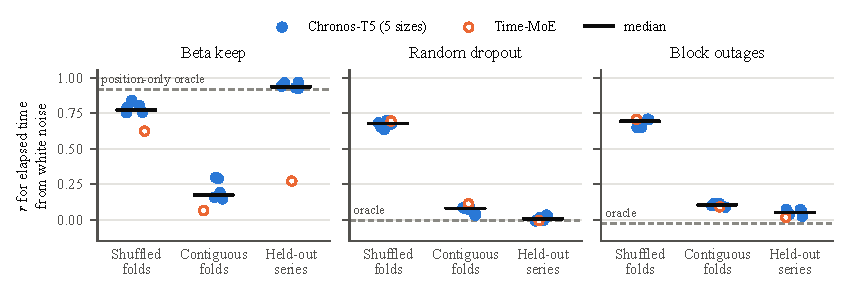
\includegraphics[width=\linewidth]{figures/fig1_trap.pdf}
  \caption{Final-layer $r$ for $\mperp$ at $p = 0.5$.
  Filled marks are white noise and open marks are real data; triangles are Time-MoE and circles are Chronos-T5.
  The dashed line is the position-only oracle.
  Under the Beta keep, held-out Chronos-T5 noise matches that oracle.
  Under random dropout and block outages the oracle is about 0, and shuffled folds still read $r = 0.63$--$0.71$ from noise.}
  \label{fig:trap}
\end{figure}

Under the Beta keep, $\mperp$ is still a smooth function of rank.
Held-out Chronos-T5 probes read it from white noise at $r = 0.92$--$0.97$, against an oracle of 0.92 (final layer).
Chronos-Bolt and Chronos-2 reach 0.96--0.97 against a patch oracle of 0.997 (main sweep, per-patch averages, best layer).
Time-MoE reaches 0.27: a causal token cannot see how many tokens follow, and the Beta curve depends on rank in the whole window.

Under random dropout and block outages the oracle is about 0, and held-out probes recover none of it from noise ($r \le 0.07$).
Shuffled folds, run for the six one-token models, still report $r = 0.63$--$0.71$ from white noise at $p = 0.5$, and $0.70$--$0.91$ on real data.
Contiguous folds fall to $0.03$--$0.12$~\citep{bergmeir2012cv,roberts2017cv}.
Shuffled folds measure smoothness; held-out series leave the position geometry, which white noise and the oracle show.

\section{What the corrected probes recover}
\label{sec:ladder}

\begin{figure}[ht]
  \centering
  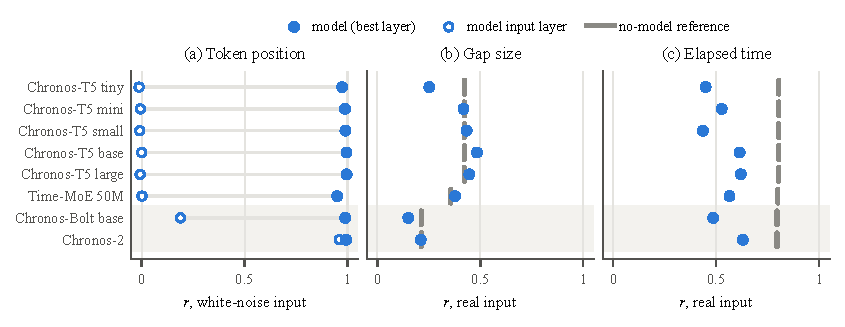
\includegraphics[width=\linewidth]{figures/fig2_v2.pdf}
  \caption{Held-out ridge probes, three draws.
  (a)~Token position from white noise under random dropout at $p = 0.5$; open marks are the input layer.
  (b)~Gap $\dt$ on real data at the same rate; grey ticks are the difference probe.
  (c)~Elapsed time under value-dependent missingness at $p = 0.7$; grey ticks are the running sum.}
  \label{fig:ladder}
\end{figure}

\begin{table}[ht]
  \caption{Held-out ridge probes; the layer is chosen on 30\% of series.
  Position is $r(k)$ from noise.
  Gap is real-minus-noise $\Delta r$ for $\dt$ at random dropout $p = 0.5$, with a 95\% interval.
  The remaining columns subtract the difference probe, then the running sum for $\mperp$ at $p = 0.7$.
  A star marks an interval that excludes 0. MLP pairs are in Appendix~\ref{app:pairs}.}
  \label{tab:main}
  \centering
  \small
  \setlength{\tabcolsep}{3.5pt}
  \begin{tabular}{lccccc}
    \toprule
    Model & Position & Gap $\Delta r$ [95\% CI] & vs difference probe & Block & Value-dependent \\
    \midrule
    Chronos-T5 tiny (8M) & 0.974 & 0.25 [0.21, 0.30] & $-0.12^{\ast}$ & $-0.17^{\ast}$ & $-0.27^{\ast}$ \\
    Chronos-T5 mini (20M) & 0.988 & 0.40 [0.30, 0.47] & $-0.00$ & $-0.11^{\ast}$ & $-0.20^{\ast}$ \\
    Chronos-T5 small (46M) & 0.990 & 0.41 [0.33, 0.49] & $+0.04^{\ast}$ & $-0.11^{\ast}$ & $-0.24^{\ast}$ \\
    Chronos-T5 base (200M) & 0.995 & 0.48 [0.36, 0.57] & $+0.06^{\ast}$ & $-0.10^{\ast}$ & $-0.17^{\ast}$ \\
    Chronos-T5 large (710M) & 0.996 & 0.44 [0.34, 0.51] & $+0.03^{\ast}$ & $-0.14^{\ast}$ & $-0.15^{\ast}$ \\
    Time-MoE (50M) & 0.950 & 0.39 [0.33, 0.45] & $+0.01$ & $-0.17^{\ast}$ & $-0.18^{\ast}$ \\
    Chronos-Bolt base & 0.989 & 0.05 [$-0.06$, 0.08] & $-0.06^{\ast}$ & $-0.14^{\ast}$ & $-0.25^{\ast}$ \\
    Chronos-2 & 0.994 & 0.13 [0.02, 0.16] & $-0.08^{\ast}$ & $-0.20^{\ast}$ & $-0.09^{\ast}$ \\
    \bottomrule
  \end{tabular}
\end{table}

Every model decodes position from white noise at $r = 0.94$--$0.996$.
For Chronos-T5 and Time-MoE the input embedding carries none; position appears in the first layers.
Chronos-2's input embedding already reaches about 0.96, from the time index on the shortened series.

The analysis plan, written before the runs and released with the code, set the gap test as decoding under random dropout at $p = 0.5$: median real-minus-noise $\Delta r > 0.10$ and an interval excluding 0.
On the planned draw, seven models passed and Chronos-2 did not.
Over three draws the six one-token models still pass.
Chronos-2's interval is then 0.13 [0.02, 0.16], and it now passes.
Chronos-Bolt passed that draw under the old per-patch averages; under the last-observation target in Table~\ref{tab:main}, three draws give 0.05 [$-0.06$, 0.08].

A difference probe on local input changes reaches $r = 0.42$ here (0.36 past-only).
Mini and Time-MoE match it, tiny falls short by 0.12, and Chronos-T5 small through large sit 0.03--0.06 above it, inside the draw-to-draw movement of the medians (about $\pm 0.05$).
Across series the gap tracks lag-1 autocorrelation (Spearman $\rho = 0.52$--$0.70$ for one-token models): a jump implies elapsed time when the series is smooth.

Under random dropout at $p = 0.7$, elapsed-time correlations are about 0.10--0.23 and the running sum is about 0.13--0.25.
Five of eight ridge intervals exclude zero and are negative; Chronos-2's ridge difference is $+0.06$, and its interval includes zero.
The MLP differences mostly include zero.
Under block outages, ridge correlations are about 0.14--0.27 and every model in Table~\ref{tab:main} falls below the running sum.
Under value-dependent missingness, ridge correlations are $0.44$--$0.63$ and the running sum is about 0.80.
The same deficit holds at $p = 0.5$ for all 32 model--probe pairs, with intervals excluding zero (Appendix~\ref{app:pairs}).
The running sum has an explicit accumulator.
The probe has to find accumulated time in one token's state.
The deficit means these probes do not read it out in that form.
On the noise inputs, the same MLP decodes essentially no elapsed time for the one-token models ($|r| \le 0.071$ across conditions).

From 8M to 710M, position decoding moves from 0.974 to 0.996, and gap $\Delta r$ from 0.25 at tiny to 0.40 at mini before flattening.
Patch medians drop series with fewer than eight patches (about 22\% of cells).

\section{Recommendations}
\label{sec:recs}

(1)~Run the probe on white noise at the same kept steps.
(2)~Evaluate on held-out series.
(3)~Report the position-only oracle; a model that matches it is reading position.
(4)~Probe gaps and elapsed time separately.
(5)~Compare with a no-model baseline built from the features you claim the model uses.
A baseline that sums the gaps tests whether the states expose that sum.

\section{Limitations}
\label{sec:limits}

Value-dependent missingness is one missing-not-at-random mechanism.
UCR series are short and univariate.
We measure representations, not forecasts.
Quantizing the difference probe's inputs, as Chronos-T5 does, changes model-minus-probe gap correlations by at most 0.015.
We do not run the NaN-on-grid input that the three Chronos models accept.

\section{Conclusion}
\label{sec:conc}

Held-out series, matched-keep noise, and a position-only oracle expose both the position curve and shuffled-fold interpolation.
Position is available from noise, and one-token gap decoding sits near a no-model probe on local value changes.
Where the values reveal the gaps, elapsed time is readable and a running sum of that probe reads more.
Leaving the missing steps on the grid gives Chronos-T5, Chronos-Bolt, and Chronos-2 the spacing as input; whether they use it is untested.
Code and per-series results: \url{https://github.com/AIpsychonaut/neurips-fmts-2026}.

\begin{ack}
No external funding was received for this work.
The author declares no competing interests.
\end{ack}

{\small
\bibliographystyle{plainnat}
\bibliography{refs}
}

\appendix

\section{Protocol}
\label{app:protocol}

Chronos-T5 states are encoder hidden states after the model's tokenizer, with the EOS position dropped.
Chronos-Bolt states are encoder states on left-padded patches; a register token is appended and then dropped before probing.
Chronos-2's \texttt{encode}, in \texttt{chronos-forecasting}~2.3.2, embeds the context patches and one future query patch, joins them, and runs the encoder once.
Hooks keep the context rows.
Time-MoE states are the inner decoder's hidden states on values $z$-scored per series.
Seeds are $42 + 1000s + 100\ell + \mathrm{round}(10p)$, plus $10^{7}$ times the draw.
Noise adds $7777777$.
The oracle uses 200 Monte Carlo draws and 50 rank bins.
Compute was about 5 GPU-hours on one NVIDIA A10G.

\section{Replication}
\label{app:replication}

On the original eight series, truncated at 400, Beta keep, $p = 0.5$, Chronos-T5-base, final layer, and shuffled folds: median $r(\mperp) = 0.821$ on real data in both bf16 and fp32.
Noise is 0.760 in bf16 (0.7597 before rounding) and 0.759 in fp32.
The submitted report was 0.821 and 0.759.

\section{Further pairs}
\label{app:pairs}

Model minus running sum for $\mperp$ at $p = 0.7$, ridge / MLP.
Every interval excludes 0.
At $p = 0.5$, all 32 model--probe pairs fall below the running sum with intervals excluding 0.
These intervals are series bootstraps for one comparison at a time.
They are not adjusted for the number of models and conditions.
Full grids are released with the code.

\begin{table}[h]
  \caption{Model minus running sum at $p = 0.7$, ridge / MLP.}
  \label{tab:appc}
  \centering
  \small
  \begin{tabular}{lcc}
    \toprule
    Model & Block outages & Value-dependent \\
    \midrule
    Chronos-T5 tiny & $-0.17^{\ast}$ / $-0.25^{\ast}$ & $-0.27^{\ast}$ / $-0.26^{\ast}$ \\
    Chronos-T5 mini & $-0.11^{\ast}$ / $-0.21^{\ast}$ & $-0.20^{\ast}$ / $-0.18^{\ast}$ \\
    Chronos-T5 small & $-0.11^{\ast}$ / $-0.22^{\ast}$ & $-0.24^{\ast}$ / $-0.24^{\ast}$ \\
    Chronos-T5 base & $-0.10^{\ast}$ / $-0.18^{\ast}$ & $-0.17^{\ast}$ / $-0.16^{\ast}$ \\
    Chronos-T5 large & $-0.14^{\ast}$ / $-0.15^{\ast}$ & $-0.15^{\ast}$ / $-0.13^{\ast}$ \\
    Time-MoE & $-0.17^{\ast}$ / $-0.22^{\ast}$ & $-0.18^{\ast}$ / $-0.23^{\ast}$ \\
    Chronos-Bolt & $-0.14^{\ast}$ / $-0.14^{\ast}$ & $-0.25^{\ast}$ / $-0.07^{\ast}$ \\
    Chronos-2 & $-0.20^{\ast}$ / $-0.15^{\ast}$ & $-0.09^{\ast}$ / $-0.10^{\ast}$ \\
    \bottomrule
  \end{tabular}
\end{table}

\newpage
\section*{NeurIPS Paper Checklist}

\begin{enumerate}

\item {\bf Claims}
    \item[] Answer: \answerYes{}
    \item[] Justification: The abstract and \S\ref{sec:intro} are supported in \S\ref{sec:trap} and \S\ref{sec:ladder}. Analyses added after the plan are labelled as such.

\item {\bf Limitations}
    \item[] Answer: \answerYes{}
    \item[] Justification: \S\ref{sec:limits}.

\item {\bf Theory assumptions and proofs}
    \item[] Answer: \answerNA{}
    \item[] Justification: No theorems.

\item {\bf Experimental result reproducibility}
    \item[] Answer: \answerYes{}
    \item[] Justification: \S\ref{sec:setup} and App.~\ref{app:protocol} give models, data selection, drop patterns, seeds, probes and references; all weights and data are public.

\item {\bf Open access to data and code}
    \item[] Answer: \answerYes{}
    \item[] Justification: Code, the analysis plan and per-series results are in the public repository linked in \S\ref{sec:conc}. UCR~2018~\citep{dau2019ucr} and the model weights are public.

\item {\bf Experimental setting/details}
    \item[] Answer: \answerYes{}
    \item[] Justification: App.~\ref{app:protocol}: ridge $\lambda=1$, GroupKFold by series, layer selection on a fixed 30\% of series.

\item {\bf Experiment statistical significance}
    \item[] Answer: \answerYes{}
    \item[] Justification: Medians over series with series-bootstrap 95\% CIs (2{,}000 resamples). \S\ref{sec:ladder} averages three keep draws. The intervals are not adjusted for the number of models and conditions (App.~\ref{app:pairs}).

\item {\bf Experiments compute resources}
    \item[] Answer: \answerYes{}
    \item[] Justification: App.~\ref{app:protocol}.

\item {\bf Code of ethics}
    \item[] Answer: \answerYes{}
    \item[] Justification: Audit of public models on a public archive; no human subjects.

\item {\bf Broader impacts}
    \item[] Answer: \answerNA{}
    \item[] Justification: Evaluation methodology for model analysis; no deployment.

\item {\bf Safeguards}
    \item[] Answer: \answerNA{}
    \item[] Justification: No high-risk release.

\item {\bf Licenses for existing assets}
    \item[] Answer: \answerYes{}
    \item[] Justification: Chronos, Chronos-Bolt and Chronos-2 are Apache-2.0. Time-MoE is Apache-2.0. The UCR archive is cited and used under its terms.

\item {\bf New assets}
    \item[] Answer: \answerYes{}
    \item[] Justification: The released code documents the protocol and regenerates every figure and table.

\item {\bf Crowdsourcing and research with human subjects}
    \item[] Answer: \answerNA{}
    \item[] Justification: None.

\item {\bf Institutional review board (IRB) approvals}
    \item[] Answer: \answerNA{}
    \item[] Justification: None.

\item {\bf Declaration of LLM usage}
    \item[] Answer: \answerYes{}
    \item[] Justification: An LLM assistant wrote experiment and analysis code and drafted text under the author's direction; the author verified all claims, numbers and citations.

\end{enumerate}


\end{document}
